\documentclass{article}
\usepackage{graphicx}
\usepackage{algorithm}
\usepackage[noend]{algorithmic}
\usepackage{subfigure}
\usepackage{amssymb, amsmath, graphicx, charter, latexsym}
\usepackage{layouts}
\usepackage[letterpaper]{geometry}
\usepackage{enumerate}
\usepackage{ragged2e}
%\usepackage{times}
\usepackage{mathtools}
%\usepackage[scaled]{helvet}
\usepackage{mathptmx}
\usepackage{verbatim}
\usepackage{listings}
\usepackage{siunitx}

\lstset{
basicstyle=\ttfamily,
}

\begin{document}

\title{\bf ECEN 689-- Real-Time Wireless Networks: Project 1\\ (Due on 2/26)}
\date{}
\author{%
Ping-Chun Hsieh\\
\texttt{lleyfede@tamu.edu}
\and
Tao Zhao\\
\texttt{alick@tamu.edu}
\and
Dongni Han\\
\texttt{handongni2015@tamu.edu}
}
\maketitle

\section*{Terminology}

In our report, we use ``server'' to denote the WiFi access point (AP), and
``client'' to denote the terminal device such as a mobile phone, a tablet, and
so on. Throughout our simulation, we let node $0$ be the server, and node $1$ be
the client, which correspond to the device A and B in the problem descriptions
respectively.

S-WiFi is the name of our application as well as our project. It stands for
Smart WiFi, or whatever you think it is.

\section*{Simulation Setup}
\begin{table}[htbp]
\centering
    \caption{Parameters of the wireless channel.}
    \vspace{2mm}
    \begin{tabular}{ | l | l | }
    \hline
    Item & Value \\ \hline
    Path loss exponent & 2.0  \\ \hline
    Shadowing deviation & \SI{4.0}{dB} \\ \hline
    Reference distance & \SI{1.0}{m} \\
    \hline
\end{tabular}
\label{table: channel}
\end{table}
Throughout the report, we consider a single wireless link between two devices, say A and B. The transmitter power level is \SI{1}{Watt}. We use the shadowing module as the wireless channel. The parameters of the channel are summarized in Table \ref{table: channel}.

\begin{table}[htbp]
\centering
\caption{Parameters of the 802.11b MAC.}
    \vspace{2mm}
    \begin{tabular}{ | l | l | }
    \hline
    Item & Value \\ \hline
    Data rate & \SI{11}{Mb/s}  \\ \hline
    Basic rate & \SI{1}{Mb/s}  \\ \hline
    PLCP data rate & \SI{1}{Mb/s}  \\ \hline 
    Preamble length & \SI{144}{bits} \\ \hline
    Slot time & \SI{20}{\mu s} \\ \hline
    SIFS & \SI{10}{\mu s} \\
    \hline
\end{tabular}
\label{table: mac}
\end{table}

For the medium access control (MAC) layer, we use the 802.11 module built in ns-2. Following the IEEE 802.11b standard, the MAC layer parameters are chosen as in Table \ref{table: mac}.


\section{Downlink Transmissions}
\label{section: downlink}
\subsection{Proposed Design in NS-2}
For downlink transmissions, the server transmits a data packet to the client periodically. As the client receives the data packet successfully, it replies an application ACK to the server.

In the S-WiFi application, we define a new packet type \lstinline|SWiFi_PKT_ACK| to measure different timings. Although the 802.11 MAC has a default ACK packet type, the default ACK frame includes no timing information or packet sequence number, which are required in timing measurement (especially in the case with automatic retry of 802.11). To be fully compatible with the original 802.11 MAC, we choose to create a new ACK in the application.

In the S-WiFi application, we define a new command ``send'', and let node 0 call the send command every \SI{10}{ms} in the Tcl domain. When the send command is called, the S-WiFi application will create a packet of size 1000 bytes and record the current timestamp, denoted by $T_s$, in the packet header as the send time in the application layer, and then send it to the client.

When the client receives the data packet and verifies the packet type in the header, it extracts the send time $T_s$ in the header of the received packet. Then, the client creates a \lstinline|SWiFi_PKT_ACK| packet with $T_s$ attached in the header, and then reply this packet to the server.

As the server receives the \lstinline|SWiFi_PKT_ACK| packet, it decodes the header and retrieves the old send time $T_s$ and checks the current timestamp upon reception. Let $T_r$ denote the current reception time. The round-trip time of a downlink transmission can be calculated by:
\begin{equation}\label{equation: rtt}
\textrm{RTT}=T_r - T_s
\end{equation}
Afterwards, the client calls a Tcl instproc (member function of a class
in Tcl's terminology) \lstinline|recv| with the data message and RTT as the
arguments. \lstinline|recv| simply stores the information into a log file.
The overall process of a downlink transmission is summarized in Figure \ref{figure: rtt}(a). 

\subsection{Simulation Results}
Under the simulation setup described above, the downlink RTT is \SI{1.625}{ms} when the distance between A and B is \SI{1}{m} and the packet size is \SI{1000}{bytes}. 
\section{Uplink Transmissions with PCF}
\label{section: uplink}
\subsection{Proposed Design in NS-2}
In uplink transmissions with PCF, the server sends out a POLL packet to
the client periodically. When the client receives the POLL packet, and has data
to be transmitted, it replies with a data packet.

Since ns-2 does not have a PCF module, we mimic the PCF behavior in the
application layer. Specifically, we define a new packet type
\lstinline|SWiFi_PKT_POLL|, and a new command ``poll'' for the S-WiFi
application. We let node 0 call the poll command every \SI{10}{ms}.
During the execution of the poll command, we create a new packet, set the packet
type \lstinline|SWiFi_PKT_POLL| and record the current time as the send time in
the packet header, and then send it out.

When the client receives a packet and finds its packet type is
\lstinline|SWiFi_PKT_POLL|, it acquires the send time, creates a new packet whose type is
data from client to server, and carries the old send time in its
header. Then it sets the packet size, fills the payload with its data message
(a predefined string in our simulation), and sends it out.

When the server receives a packet and finds it is a data packet from client to
server, it decodes the data message and gets the old send time $T_\text{s}$ from
the packet header. Besides, upon receiving the packet, the server gets the current timestamp denoted by $T_r$. The RTT of a uplink transmission can be calculated as in (\ref{equation: rtt}).
To output the RTT information into a log file, the client calls \lstinline|recv| with the data message and RTT as the arguments. The process of a uplink transmission is summarized in Figure \ref{figure: rtt}(b).

\subsection{Simulation Results}
Under the simulation setup described in previous sections, the uplink RTT is \SI{1.625}{ms} when the distance between A and B is \SI{1}{m} and the packet size is \SI{1000}{bytes}. \\

\begin{figure}[htbp]
\centering
\subfigure[Downlink round-trip time.]{
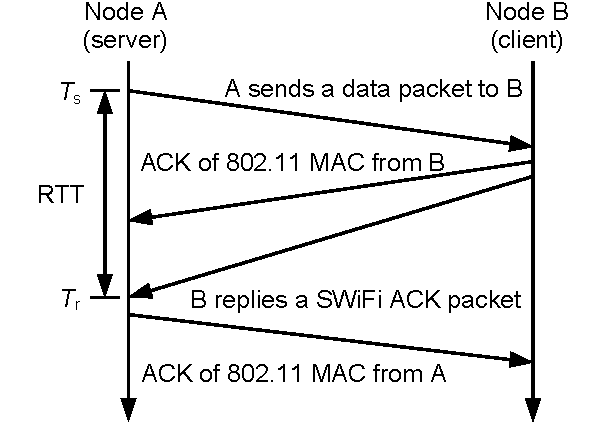
\includegraphics[scale = 0.7]{downlink_rtt.pdf}}
\subfigure[Uplink round-trip time.]{
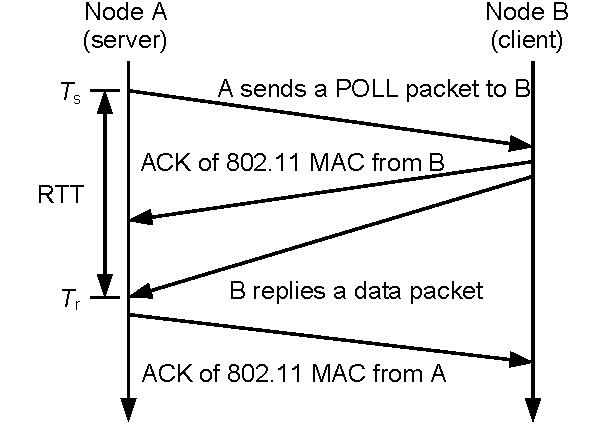
\includegraphics[scale = 0.7]{uplink_rtt.pdf}}
\caption{Round-trip time when node A and node B are close to each other.}
\label{figure: rtt}
\end{figure}

\section{Transmission Reliability}
\subsection{Implementation}
Based on the design in Section \ref{section: downlink} and \ref{section: uplink}, we are able to measure reliability by simply editing the Tcl file. We first add two global variables in the Tcl domain: \lstinline|num_trans| for the total number of packets generated by the client and \lstinline|n_rx| to count the number of successful transmissions. In the instproc \lstinline|recv|, we increase \lstinline|n_rx| by 1. At the end of simulation, the client calls a Tcl instproc \lstinline|stat| with \lstinline|n_rx| and \lstinline|num_trans| as the input arguments. \lstinline|stat| simply calculates the reliability and outputs the results into a data file. One important thing to note is that to obtain the real channel reliability, we need to disable the automatic retry function built in 802.11 MAC. This can be done by setting the \lstinline|ShortRetryLimit_| and \lstinline|LongRetryLimit_| to be 0 in the Tcl domain.

\subsection{Simulation Results}
Figure \ref{figure: reliability}(a) shows the channel reliability of downlink transmissions with distance between A and B ranging from \SI{1}{m} to \SI{2000}{m}. In each simulation run, the server generates $10^4$ data packets in total. When the distance is less than \SI{500}{m}, the reliability remains close to $100\%$. The reliability drops to about $56.7\%$ at \SI{1000}{m} and to $3.9\%$ at \SI{2000}{m}. Due to the symmetry of uplink and downlink transmission pattern, uplink has almost the same channel reliability as downlink, as shown in Figure \ref{figure: reliability}(b).

\begin{figure}[htbp]
\centering
\subfigure[Reliability of downlink transmissions.]{
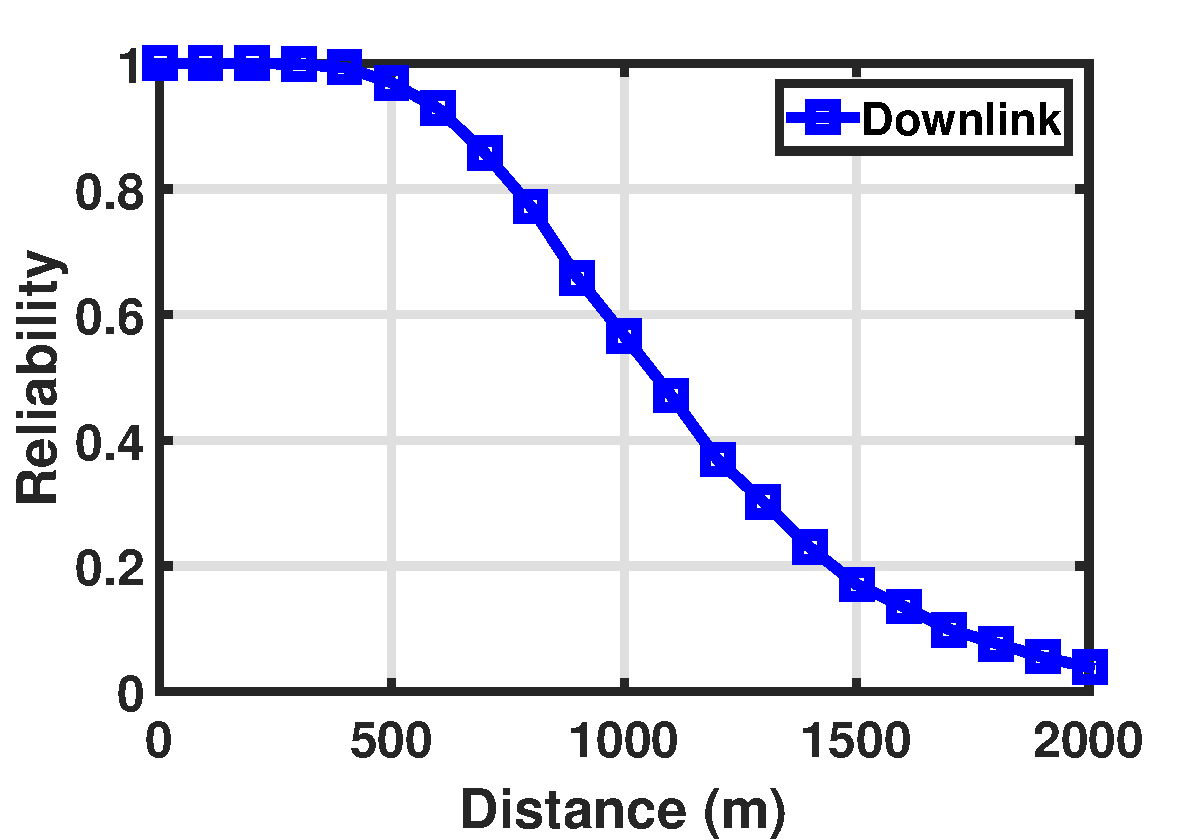
\includegraphics[scale=0.35]{p3_downlink.pdf}}
\subfigure[Reliability of uplink transmissions.]{
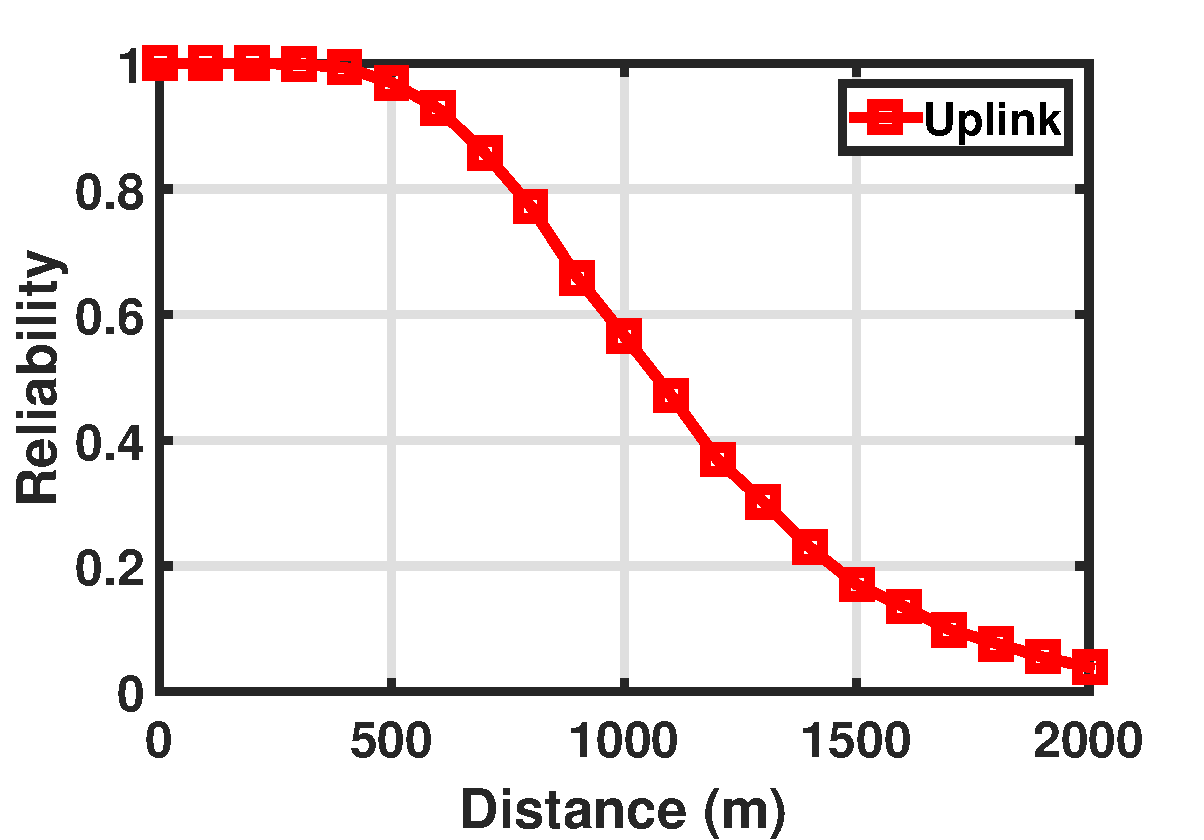
\includegraphics[scale=0.35]{p3_uplink.pdf}}
\caption{Reliability versus distance.}
\label{figure: reliability}
\end{figure}

\section{Measuring Delays}
\subsection{Implementation}
To measure the delay of packet delivery, we first enable the automatic retry function in 802.11 MAC. This can be done by setting the \lstinline|ShortRetryLimit_| and \lstinline|LongRetryLimit_| in the 802.11 MAC. Recall the process of downlink transmission described in Section \ref{section: downlink}. Let $T_{send}$ still be the time at which the server creates a data packet intended for the client, and let $T_{recv}$ be the time when the server receives the corresponding \lstinline|SWiFi_PKT_ACK| from the client. The packet delay is simply calculated by $T_{recv}-T_{send}$. However, since it is possible that a node takes multiple transmissions to deliver one packet successfully, packet delay is greater than or equal to RTT. For example, in Figure \ref{figure: downlink delay}, node A delivers a data packet after 1 retry and node B replies a S-WiFi ACK successfully using two transmissions.

\begin{figure}[htbp]
\centering
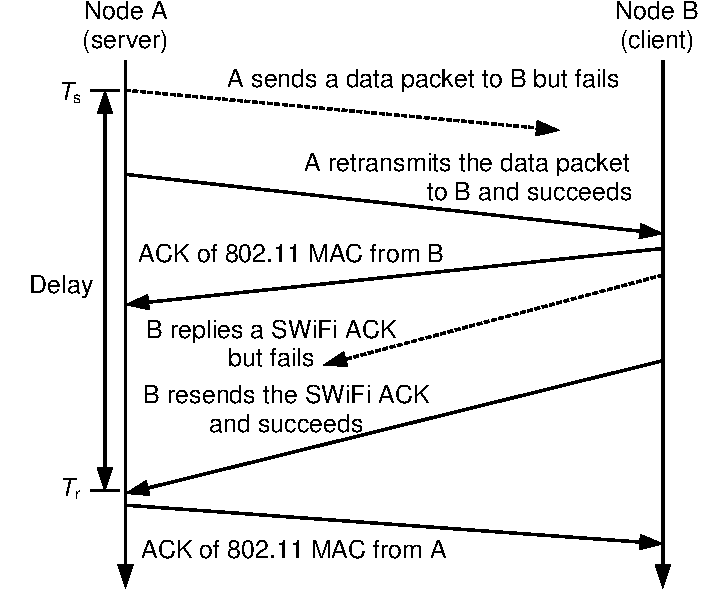
\includegraphics[scale = 0.7]{downlink_delay.pdf}
\caption{Downlink packet delay with automatic retransmissions.}
\label{figure: downlink delay}
\end{figure}

Similarly, for uplink transmission, let $T_{send}$ still be the time when the server creates a \lstinline|SWiFi_PKT_POLL| packet and $T_{recv}$ be the time when the server receives the data packet sent by the client. Then, the packet delay can again be calculated by $T_{recv}-T_{send}$. As an exmaple, Figure \ref{figure: uplink delay} shows the packet delay of uplink transmission with automatic retry.

\begin{figure}[htbp]
\centering
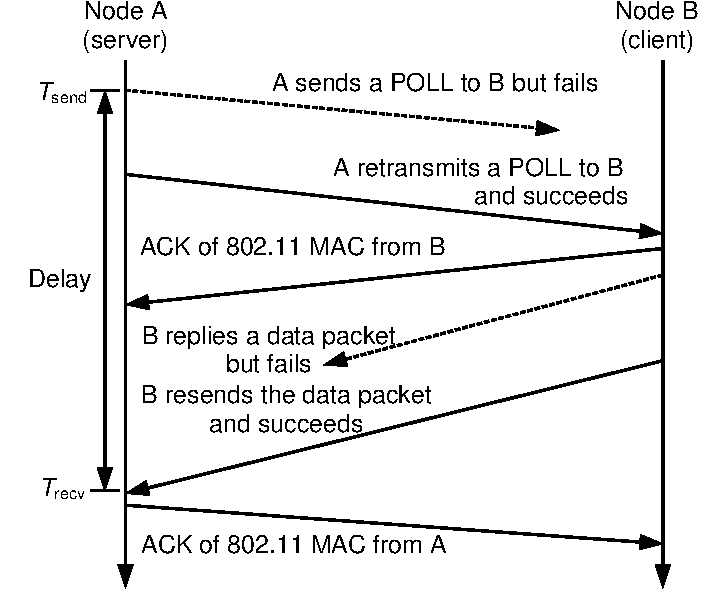
\includegraphics[scale = 0.7]{uplink_delay.pdf}
\caption{Uplink packet delay with automatic retransmissions.}
\label{figure: uplink delay}
\end{figure}

\subsection{Simulation Results}
The packet delay is measured under the channel reliability of about $55\%$. From Figure \ref{figure: reliability}(a) and \ref{figure: reliability}(b), we choose the distance between A and B to be \SI{1000}{m} for both uplink and downlink transmission. The length of a slot is chosen to be one RTT, which is \SI{1.625}{ms} given in Section \ref{section: downlink} and \ref{section: uplink}. In each simulation run, the server generates a packet every two time slots, and sends $10^4$ data packets to the client in total.

Figure \ref{figure: downlink delay cdf} shows the cumulative distribution function of delays of downlink transmissions with automatic retry limit from 0 to 5. When the retry limit is 0, the delay is about \SI{1.6}{ms} for all the packets. This is because every packet has to be either delivered in one transmission or simply dropped by the 802.11 MAC. When the retry limit is 1, each node might take either one or two transmissions to deliver a packet. Moreover, some packets might be queued in the MAC layer so that the real send timestamp in the MAC layer can be much larger than the packet generation timestamp in the application layer. When the retry limit is greater than or equal to 2, the {queueing delay} dominates the delay of packet delivery. 

Similar to downlink, uplink transmissions exhibit the same delay pattern as shown in Figure \ref{figure: uplink delay cdf}. {\bf [EXPLAIN why uplink has smaller delays]}
Table \ref{table: average delay} shows the average packet delay of both downlink and uplink transmissions with different retry limits.  

\begin{figure}[htbp]
\centering
\subfigure[CDF of delay with retry limit 0 and 1.]{
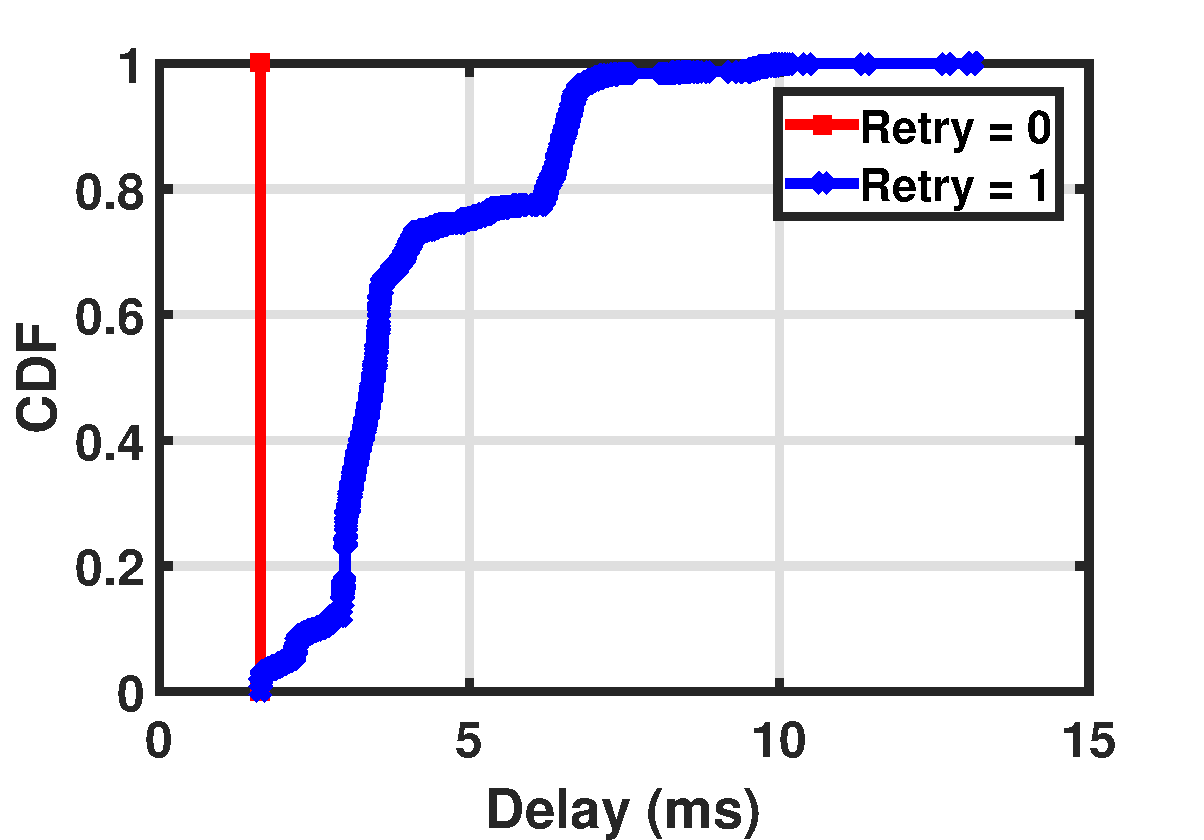
\includegraphics[scale=0.35]{p4_downlink_1.pdf}}
\subfigure[CDF of delay with retry limit 2, 3, 4, and 5.]{
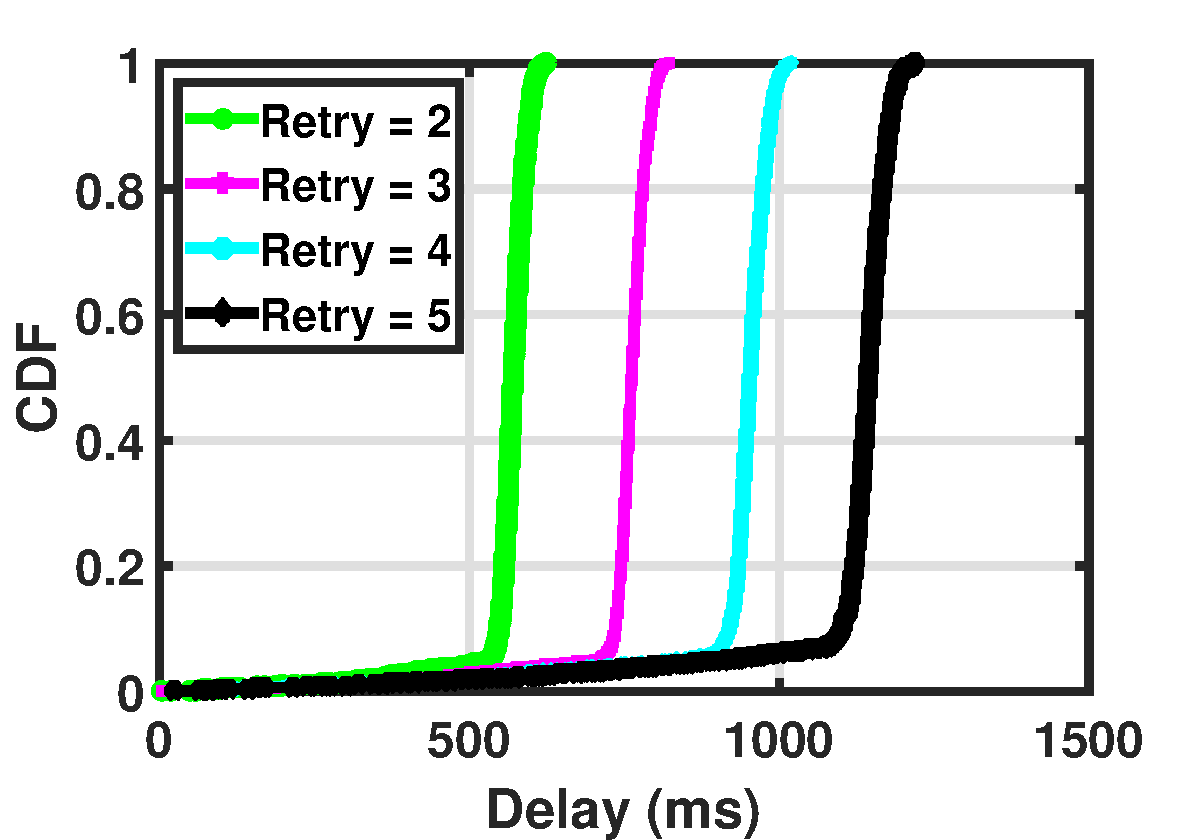
\includegraphics[scale=0.35]{p4_downlink_2.pdf}}
\caption{Probability distribution of packet delay of downlink transmission.}
\label{figure: downlink delay cdf}
\end{figure}

\begin{figure}[htbp]
\centering
\subfigure[CDF of delay with retry limit 0 and 1.]{
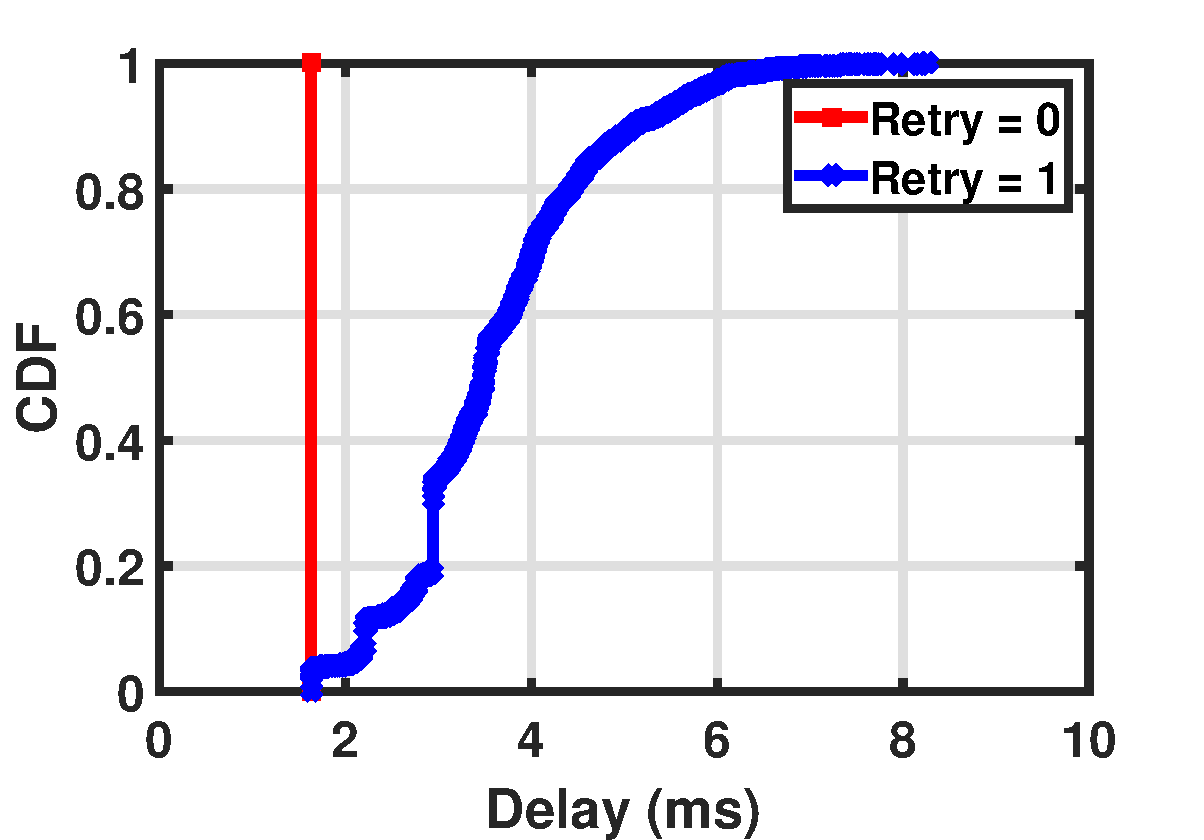
\includegraphics[scale=0.35]{p4_uplink_1.pdf}}
\subfigure[CDF of delay with retry limit 2, 3, 4, and 5.]{
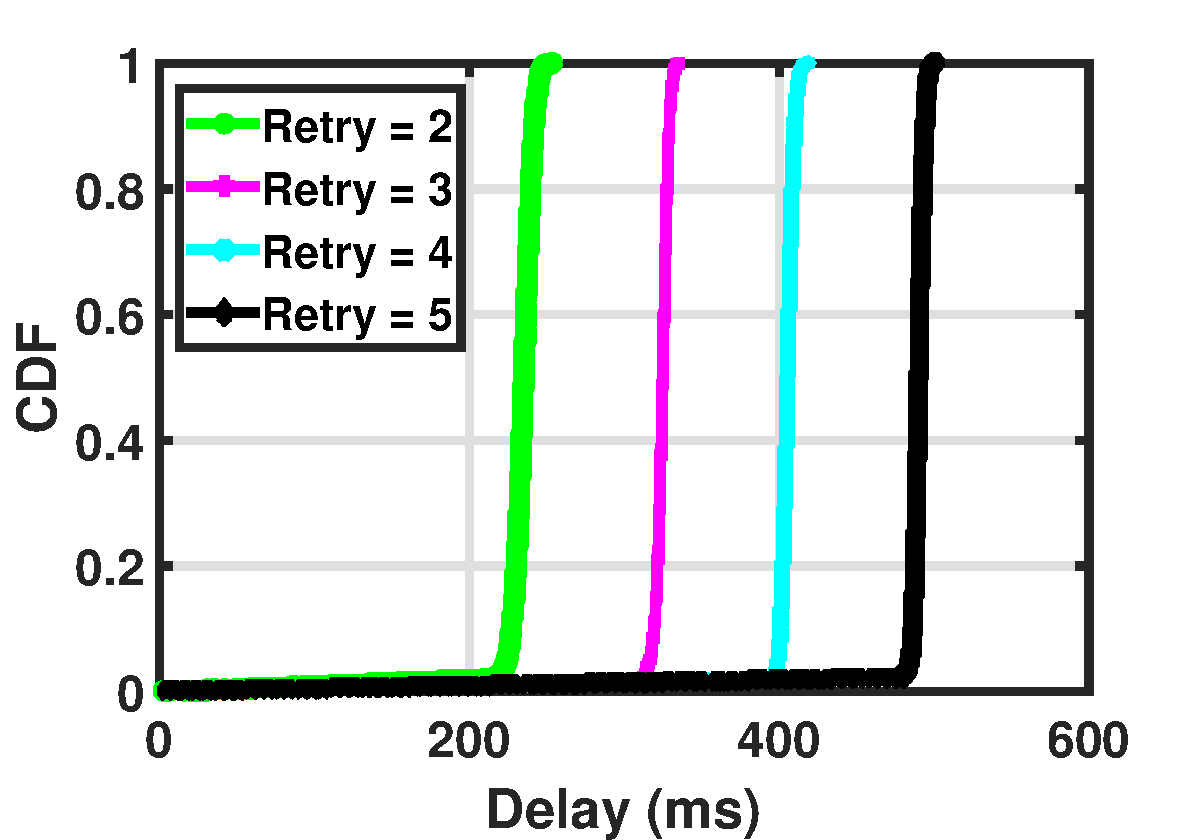
\includegraphics[scale=0.35]{p4_uplink_2.pdf}}
\caption{Probability distribution of packet delay of uplink transmission.}
\label{figure: uplink delay cdf}
\end{figure}


\begin{table}[htbp]
\centering
    \caption{Average packet delay of downlink and uplink transmissions.}
    \vspace{2mm}
    \begin{tabular}{ | c | l | l | }
    \hline
    Retry limit & Downlink & Uplink \\ \hline
    0& \SI{1.631}{ms} & \SI{1.631}{ms} \\ \hline
    1 & \SI{4.589}{ms}  & \SI{4.174}{ms} \\  \hline
    2 & \SI{561.2}{ms} & \SI{232.0}{ms} \\  \hline
    3 & \SI{747.4}{ms}  & \SI{320.7}{ms} \\  \hline
    4 & \SI{931.6}{ms}  & \SI{400.8}{ms} \\  \hline
    5 &  \SI{1113}{ms} & \SI{483.8}{ms} \\ 
    \hline
\end{tabular}
\label{table: average delay}
\end{table}

\section{Preferences for Final Report}
We prefer topic 2 to topic 3, and prefer topic 3 to topic 1. ($2 \succ 3 \succ 1$)


\end{document}
